%for a more compact document, add the option openany to avoid
%starting all chapters on odd numbered pages
\documentclass[12pt,openany,dvipsnames]{cmuthesis}
\usepackage{etoolbox}
\usepackage{fancyvrb}
\usepackage{times}
\usepackage{dashrule}
\usepackage{proof-dashed}
\usepackage[show]{ed}
\usepackage{fullpage}
\usepackage{graphicx}
\usepackage{xcolor}
\usepackage{tikz}
\usepackage{rotating}
\usetikzlibrary{arrows,decorations.pathmorphing,backgrounds,fit}
\usepackage{amsthm}
\usepackage{amsmath}
\usepackage{latexsym}
\usepackage{amssymb}            % for \multimap (-o)
\usepackage{stmaryrd}           % for \binampersand (&), \bindnasrepma (\paar)
\usepackage{wasysym}            % for \ocircle
\usepackage[numbers,sort]{natbib}
\usepackage[backref,pageanchor=true,plainpages=false, pdfpagelabels, bookmarks,bookmarksnumbered,
%pdfborder=0 0 0,  %removes outlines around hyper links in online display
]{hyperref}
\usepackage{doi}
\usepackage{subfigure}

% Approximately 1" margins, more space on binding side
%\usepackage[letterpaper,twoside,vscale=.8,hscale=.75,nomarginpar]{geometry}
%for general printing (not binding)
\usepackage[letterpaper,twoside,vscale=.8,hscale=.75,nomarginpar,hmarginratio=1:1]{geometry}

\hypersetup{colorlinks=true,citecolor=blue,urlcolor=blue,linkcolor=black}

% Theorems
\newtheorem{theorem}{Theorem}[chapter]
\newtheorem{lemma}[theorem]{Lemma}
\newtheorem{proposition}[theorem]{Proposition}
\newtheorem{definition}[theorem]{Definition}

% Entailment
\newcommand{\EEq}{\approx}

% Formulae
\newcommand{\Top}{\top}
\newcommand{\Bot}{\bot}
\newcommand{\Or}{\vee}
\renewcommand{\And}{\wedge}
\newcommand{\Imp}{\supset}
\newcommand{\All}{\forall}
\newcommand{\Ex}{\exists}

% Sequents
\newcommand{\CSeq}[3]{{#1}~|~{#2} \Longrightarrow {#3} \mathstrut}

% Derivations
\newcommand{\C}{\ensuremath{\mathcal{C}}}
\newcommand{\D}{\ensuremath{\mathcal{D}}}
\newcommand{\E}{\ensuremath{\mathcal{E}}}

% Brackets
\newcommand{\Set}[1]{\left\{#1\right\}}
\newcommand{\ASet}[1]{\left<#1\right>}
\newcommand{\BSet}[1]{\left[#1\right]}


%%% Local Variables:
%%% mode: latex
%%% TeX-master: "thesis"
%%% End:


\newtoggle{dev}
%\togglefalse{dev}
\toggletrue{dev}

\iftoggle{dev}{
  \includeonly{chapter-intro}
}

\iftoggle{dev}{
  \draftstamp{\rm \today}{\rm DRAFT}
}

\begin {document}
\frontmatter

\pagestyle{empty}

\title{
  {\bf The Polarized Inverse Method}
  %{\it (First committee draft)}
}
\author{Sean McLaughlin}
\date{\today}
\Year{2015}
\trnumber{revision 0.0.1}

\committee{
  Frank Pfenning, Chair \\
  Jeremy Avigad \\
  Robert Harper \\
  Dale Miller, INRIA-Saclay \& LIX/Ecole Polytechnique \\
  Andr\'e Platzer
}

\support{This research was supported by
National Science Foundation grant NSF-0716469 (\emph{Manifest Security}) and
Air Force Research Laboratory grant FA87500720028 (\emph{Accountable Information
  Flow via Explicit Formal Proof})}

\disclaimer{Any opinions, findings, conclusions or recommendations
  expressed in this publication are those of the author and do not
  necessarily reflect the views of any sponsoring institution or
  government.}

\keywords{automated theorem proving, intuitionistic logic, inverse
  method, focusing, polarization, linear logic, ordered logic,
  constraint programming}

\maketitle

%%% Local Variables:
%%% mode: latex
%%% TeX-master: "thesis"
%%% End:
             %
%\begin{dedication}
  To my parents.
\end{dedication}

%%% Local Variables:
%%% mode: latex
%%% TeX-master: "thesis"
%%% End:


\pagestyle{plain}

%
\begin{abstract}
Non-classical logics provide a flexible means for describing and
reasoning about diverse computational phenomena.
\emph{Intuitionistic logic} provides a foundation for constructive
mathematics and is the
basis of numerous logical frameworks and proof assistants which are
used to reason about programs.  \emph{Modal logics} permit succinct
reasoning about possible worlds, which has applications to
authorization and distributed computing.  \emph{Linear logic} and
\emph{ordered logic}, with their interpretation of hypotheses as
resources, are used to study stateful and concurrent systems.

Theorem proving in these logics is typically difficult. For example,
while in classical logic the decision problem for the propositional
fragment is NP-complete, intuitionisitic logic is PSPACE-complete,
while even fragments of propositional linear logic are undecidable.
Nevertheless, it is fundamental to the adoption of such expressive
logics that we develop practical theorem proving tools.

We describe a general method for building efficient theorem provers for
non-classical logics called the \emph{polarized inverse method}.  The
\emph{generality} of our approach comes from the use of the inverse method, a
well-known proof search strategy for cut-free sequent calculi, and the use of
\emph{constraints} for delaying the results of costly computations.
\emph{Efficiency} comes from the relatively novel proof-theoretic methods of
\emph{focusing} and \emph{polarization} as well as more standard techniques
such as redundancy elimination.

Throughout the thesis we will demonstrate by example that the inverse
method, augmented with constraints, focusing, and polarization, forms
a strong foundation for efficient theorem proving in non-classical
logics.  We give support to our claims by describing an implementation of
a theorem prover called \emph{Imogen} for propositional and first-order logic,
first-order logic with equality, some first-order some standard
intuitionistic modal logics (K, T, K4, S4, S5), lax logic,
Pfenning and Davies' computational modal logic, linear and ordered
logic).
We find in empirical tests
that Imogen compares favorably with existing implementations.  For
first-order logic with equality, ordered logic and some modal logics,
Imogen is the first and only existing implementations.
\end{abstract}

%%% Local Variables:
%%% mode: latex
%%% TeX-master: "thesis"
%%% End:


\iftoggle{dev}{}{\tableofcontents}

\mainmatter

%% Double space document for easy review:
%\renewcommand{\baselinestretch}{1.66}\normalsize
\chapter{Introduction}
\label{chapter-introduction}

This thesis describes advances in theorem proving in first-order intuitionistic
logic.  We show that the \emph{polarized inverse method}, a focused, bottom-up
proof search procedure, combined with \emph{constraints} yields an efficient,
general, and practical tool for some kinds of intuitionistic automated
reasoning.To provide evidence for our claim of efficiency, we built a framework
based on the polarized inverse method with constraints called \emph{Imogen}.
Imogen is competitive with the best existing theorem provers in pure
propositional logic.  It is the best performing implementation for pure
first-order logic.  To provide evidence for our claim of generality, we use
Imogen to build theorem provers for intuitionistic modal logic, linear logic,
and ordered logic.  To provide evidence for our claim to practicality, we used
the framework to build useful tools for analyzing networking and authorization
in the Amazon Web Services (AWS) cloud.

\subsubsection*{Constraints}

The main contribution of the thesis is the use of \emph{constraint domains}
together with the polarized inverse method. Pure first-order logic treats
function symbols as \emph{uninterpreted}; any facts about the symbols are
explicit in the formula.  Constraint domains make the behavior of some function
symbols implicit.  For example, if we are reasoning about integers, the ``+''
symbol can be interpreted as addition without explicitly giving axioms defining
addition in the formula itself.  As another example, the domain of bit-vectors
are particularly useful in applications to computer networks.  For example,
given three 32-bit vectors, the first ($\Ip$) representing an IP address, the
second two representing the two components of a CIDR range ($\Base$, $\Mask$),
the following formula defines a predicate $\Matches$, which indicates that the
IP belongs to the CIDR range:

\[
\All\Ip, \Base,\ \Mask: \BV_{32}.\
  \Matches(\Ip, \Base, \Mask) \Iff \Ip \BvAnd \Mask = \Base\BvAnd\Mask
\]

\noindent
Here the domain consists of the sort $\BV_{32}$ of bit-vectors of length 32,
the bitwise ``and'' operator (\&), and equality on bit-vectors.  An IP address
$\Ip$ matches a CIDR range if the bitwise ``and'' of $\Ip$ with the subnet
mask $\Mask$ is identical to the CIDR start address $\Ip$ ``and''-ed with
$\Mask$.  For example, we would expect the following to be provable:

\[
\begin{array}{l}
  \Matches(10.0.10.10, 10.0.0.0, 255.255.0.0)
  \\[5pt]
  \Not\Matches(10.1.10.10, 10.0.0.0, 255.255.0.0)
  \\[5pt]
  \All\Ip, \Base: \BV_{32}.\
  \Matches(\Ip, \Base, 255.255.255.255) \Imp \Ip = \Base
\end{array}
\]

\noindent
We will use constraint like these extensively in our case
study where we apply these methods to analyzing networks in the
AWS cloud in Chapter~\ref{chapter-aws}.

Constraints do not change what is expressible in first-order logic.  Any formula
expressible with constraints is expressible without them.  Continuing with the
bit-vector example, we can first encode bit-vectors of length 32 as functions
$\Set{0, \ldots, 31} \to \Set{0, 1}$.  Then we can define

\[
(f\,\&\,g)(N) \Eqdef f(N)\,\&\,g(N)
\]

\noindent where the second $\&$ is the boolean
``and''.  Equality would be defined extensionally on bit-vectors;
\[f = g \Iff \All n\in\Set{0,\ldots, 31}.\ f(n) = g(n)\] where the second $=$ is
equality on the set $\Set{0,1}$.  Indeed, some classical first-order theorem
provers take this approach, since it does not require changing the
implementation.  However, we show that, at least for the
inverse method, using constraints is a far more efficient approach to
domain-specific reasoning.

\subsubsection*{Why Intuitionistic Logic?}

This work exclusively studies \emph{intuitionistic} logics.  Intuitionistic
logic has been largely ignored by the applied theorem proving community.  There
are good reasons for this; it's much more difficult to prove theorems in
intuitionistic logic than in classical logic.  The propositional case, for
example, is PSPACE-complete vs. NP-complete for classical logic.  Classical
logic has beautiful normal forms that lead naturally to simple algorithms like
DPLL that have in recent years solved astonishingly large SAT problems, and are
applied all over industry, particularly in hardware and software verification.
First-order classical logic has even nicer normal forms, due to tricks like
Skolemization, that lead again to efficient algorithms like resolution and
paramodulation.  In contrast, but for to our knowledge there are no intuitionistic
theorem provers in industrial use is there are no existing theorem provers that
efficiently handle equality in intuitionistic logic.   not necessarily
clear what you gain from
intuitionism.

In our view, the one way in which classical theorem provers are lacking is in
the evidence they give for the truth of a proposition.  Theorem proving in
classical logic is generally based on refutation; the formula is negated, and
the resulting formula is proved unsatisfiable, which indirectly implies the
original proposition is true.  While we do not doubt the consistency of
the logic, the generated resolution proofs, for example, only show that a
contradiction was obtained, and it is difficult to mine such a proof for
human-digestible justification.

In contrast, intuitionistic logic has a beautiful proof theory that corresponds
to a simple programming language.  As a result, it is possible to generate
understandable evidence that demonstrates the truth of a proposition.  For some
applications, knowing \emph{why} a proposition is true as important as knowing
\emph{that} it is true (cf. Chapter~\ref{chapter-aws}).  For a simple example,
consider the SMT-LIB program shown in Figure~\ref{figure.z3-path}.  It defines
the the type of nodes with three elements $a, b, c$ and predicates \textsf{edge}
and \textsf{path}.  Edges are atomic.  A path is either an edge, or a
combination of two paths that share an endpoint.  Then it defines edges between
$a, b$ and $b, c$.  Finally, it asks whether there's a path between $a$ and $c$.
Imogen Z3, an industrial-strength SMT solver finds the 3700 byte refutation
proof shown in Figure~\ref{figure.z3-proof}.  The equivalent constructive proof
in Imogen is

\[
\begin{array}{rl}
  &\lambda H1: \forall x\ y.\ edge(x, y) \Imp path(x, y). \\
  &\lambda H2: \forall x\ y\ z.\ path(x, y) \Imp path(y, z) \Imp path(x, z).\\
  &\lambda H3: edge(a, b). \\
  &\lambda H4: edge(b, c). \\
  &\hspace{1em}  H2\ a\ b\ c\ (H1\ a\ b\ H3)\ (H1\ b\ c\ H4)
\end{array}
\]

\begin{figure}
  \VerbatimInput[frame=lines, fontsize=\footnotesize]{figs/z3-path.smt2}
  \caption{Paths in a graph}
  \label{figure.z3-path}
\end{figure}

\begin{figure}
  \VerbatimInput[frame=lines, fontsize=\tiny]{figs/z3-proof.txt}
\caption{Z3 Proof}
\label{figure.z3-proof}
\end{figure}

Our intention is not to single out Z3 as a poor example of proof objects, but to
emphasize that classical refutation proofs have less useful information than
intuitionistic proofs.  While this fact has been a matter of philosophical
discourse for over well over a century, its \emph{usefulness} in building
useful analysis tools has been under-appreciated.  For example, constructive
proofs like the one shown above can be processed into a form
that is helpful in debugging, e.g. complicated authorization policies.

\section{Overview of the Thesis}

\begin{quote}
\textbf{Thesis Statement:} The polarized inverse method, augmented with
general constraint domains, is an effective and practical method of
automated reasoning in intuitionistic logics.
\end{quote}

To begin, in Chapter~\ref{chapter-prop} we will describe the polarized inverse
method in detail for intuitionistic propositional logic.  While the
propositional fragment lacks both constraints and quantifiers, it demonstrates
the primary theorem proving algorithm in its simplest form.  Besides showing the
calculus and proving soundness and completeness, we show a number of
optimizations that make our implementation competitive with the best existing
solvers.  Foremost among the optimizations are a series of ``polarity
disciplines'' that we call \emph{logical optimizations}.  The defining feature
of logical optimizations is that they operate only on the input formula, and are
independent of a given inverse method implementation.

In Chapter~\ref{chapter-fol} we extend the propositional prover with first-order
quantifiers.  The completeness theorem is more complicated, but similar in
spirit.  We demonstrate the effectiveness of our base method on problems from
the TPTP library.  Our implementation solves more first-order problems than any
existing prover for intuitionistic logic.

Chapter~\ref{chapter-constraints} is the main theoretical contribution of the
thesis.  We describe how to add constraints to the polarized inverse method and
prove soundness and completeness results.  The proofs are parameterized on a
given constraint domain.  We show that the domain needs only a small number of
reasonable properties (transitivity of entailment, for example) for the theorems
to work.  To finish the chapter we add bitvector and finite domain constraints
to the first-order prover from Chapter~\ref{chapter-fol}.

Chapter~\ref{chapter-aws} is a case study in using our method on a real-world
problem encountered by the author in industry: verifying properties of
cloud networking on Amazon Web Services (AWS).

Chatper~\ref{chapter-modal} shows how to apply constraints to obtain theorem
provers for some intuitionistic modal logics.

Chatper~\ref{chapter-sub}, joint work with Jason Reed, shows how to apply
constraints to obtain theorem provers for linear and ordered logic.

\begin{figure}[H]
  \begin{center}
    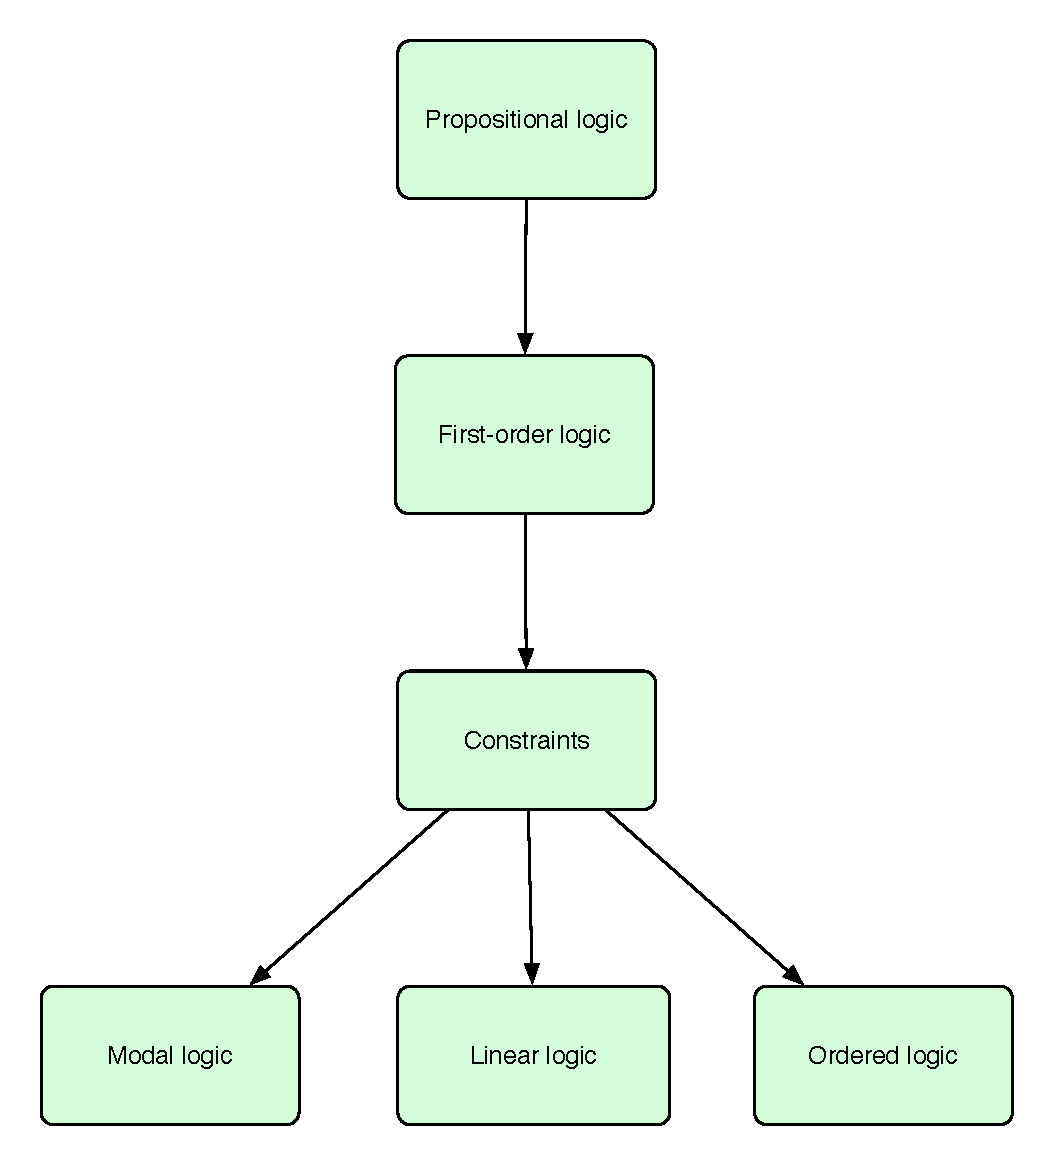
\includegraphics[scale=0.50]{figs/logics.eps}
  \end{center}
  \caption{Logics}
  \label{figure.logics}
\end{figure}

\section{Related work}

Constraints are nothing new in the literature.  Constraint logic programming and
satisfiability modulo theories (SMT) are devoted to the study of the interplay
between general logical reasoning and reasoning in constraint domains.  This
research differs from existing work in a couple of ways.  First, we are
considering full first-order intuitionistic logic as our base logic.  Constraint
logic programming remains, for all its improvements over Prolog's simple
operational semantics, a search and optimization procedure.  It can not be used
for general theorem-proving.  SMT comes closer, in that it combines solvers for
various constraint domains with classical first-order logic, though support for
arbitrary quantifier nesting is scant.  Vampire~\cite{Riazanov.1999.CADE} is the
best existing first-order classical theorem prover at the time of writing.  It
supports constraints by automatically adding (incomplete) axiomitizations of the
domains to input formulas.  Besides the obvious difference that Vampire is based
on classical logic, while our work deals with intuitionistic logic, we build
constraints into the core reasoning mechanism.


%%% Local Variables:
%%% mode: latex
%%% TeX-master: "thesis"
%%% End:

\chapter{Propositional Logic}
\label{chapter-prop}

Intuitionistic propositional logic (IPL) is the starting point for our
investigations into a uniform proof procedure for intuitionistic logics, and is
a sub-logic of all logics in later chapters.  As it involves neither quantifiers
nor constraints, it is the simplest logic we will consider.
Even so, it poses some interesting challenges, and motivates our choice of the
polarized inverse method as a proof search strategy.

\section{Preliminaries}

In this section we quickly review some background material and notations.

\paragraph{Multisets.}

Let $\cU$ be a set. A \emph{(finite) multiset} of $\cU$
is a function $f$ from
$\cU$ to $\Nat$ where $f(x)=0$ for all but a finite number of elements of
$\cU$.  The empty multiset, written $\cdot$ or $\emptyset$ is the
function $\lambda x.\ 0$. If $f$ is a multiset then $f, x$ is a multiset
where $(f, x) (x) = f(x)+1$ and $(f, x) (y)=f (y)$ when $x\neq y$.
If $f$ and $g$ are multisets, then $f\Union g$ is a multiset where
$(f\Union g) (x) = f(x)+g(x)$.  When we are writing both set and multiset union
in the same part of the text, we will use $X \uplus Y$ for multiset union.
The number of elements in a set or multiset $\Gamma$ is written $\Card{\Gamma}$.

\paragraph{Ordered sequences.}

If $\cU$ is a set, a \emph{sequence} of $\cU$ is either empty (written $[]$)
or has the form $x:S$ where $x\in \cU$ and $S$ is a sequence of $\cU$.
We abbreviate $x_1 : x_2 : \cdots : x_n : []$ as $[x_1,\ldots,x_n]$.

\paragraph{Notations.}

If $\cU$ is a set, let $\PSet{\cU}$ be the powerset of $\cU$ and $\SSet{\cU}$ be
the set of ordered sequences of elements of $\cU$.  $\SSet{\cU}_n$ is the
set of sequences of $X$ with length $n$.

\section{Sequent calculus}

% \begin{quote}
%   \textit{We define the backward calculus $\LJ$ for
%     IPL, and remind the reader of some important properties.}
% \end{quote}

% \noindent

\begin{definition}[Formulas]
  Let $\Atoms$ be an infinite set of symbols, called \emph{atoms}.
  Formulas of IPL are
  \[
  \mbox{Formulas } A ::= p \Sep A \And A \Sep \Top \Sep A \Or A
  \Sep \Bot \Sep A \Imp A
  \]
  where $p\in\Atoms$ and $\And$, $\Or$, $\Imp$, $\Top$, $\Bot$
  signify conjunction, disjunction, implication, truth, and falsehood
  respectively.
  Formulas of the first kind are called \emph{atomic}.
  Derived connectives for negation and bi-implication are
  \[
  \begin{array}{rl}
    \Not A &:= A \Imp \Bot \\
    A \Iff B &:= (A \Imp B) \And (B \Imp A).
  \end{array}
  \]
\end{definition}



\subsection{Rule generation}

\subsection{Polarization strategies}

Given an un-polarized input formula, the minimal polarization will sometimes
yield bad operational behavior in the inverse method.  For a simple example,
consider the trivial formula $(A \Or A) \Imp (A \Or A) ⊃ \ldots \Imp A$.

\newcommand{\Ps}{P(\vec{s}\,)}
\newcommand{\Pt}{P(\vec{t}\;)}
\newcommand{\Pu}{P(\vec{u}\,)}
\newcommand{\Pv}{P(\vec{v}\,)}

To verify the internal integrity (soundness and completeness) of $\C$, we prove the standard
cut elimination and identity properties.

\begin{theorem}[Identity] For any $\Phi, \Gamma, A$, \[\CSeq{\Phi}{\Gamma, A}{A}\].\end{theorem}
\begin{proof}
Induction on $A$.  Most cases are simple uses of the induction hypotheses.  We
show some representative cases.
\begin{description}
\item[Case] $A = E$.  By entailment rules id and $\And_2$, we have $\Phi\And E\models E$.
Therefore
\[
\infer[$E-L$]{\CSeq{\Phi}{\Gamma, E}{E}}{\infer[$E-R$]{\CSeq{\Phi\And E}{\Gamma}{E}}{\Phi\And E \models E}}
\]

\item[Case] $A = \Ps$.  By entailment rules refl and vec, we have $\Phi\models \vec{s}\EEq\vec{s}$.
Therefore
\[
\infer[$init$]{\CSeq{\Phi}{\Gamma, \Ps}{\Ps}}{\Phi\models\vec{s}\EEq\vec{s}}
\]

\item[Case] $A = \All x.~B(x)$
\[
\infer[\All$-R$]{\CSeq{\Phi}{\Gamma, \All x.~B(x)}{\All x.~B(x)}}{\infer[\All$-L$]{\CSeq{\Phi}{\Gamma, \All x.~B(x)}{B(a)}}{\deduce{\CSeq{\Phi}{\Gamma, \All x.~B(x), B(a)}{B(a)}}{\D'}}}
\]

where $\D'$ exists by induction hypothesis.
\end{description}
\end{proof}

\begin{theorem}[Admissibility of Cut]\label{thm:cut-admissible}
The following rule is admissible:

\[
\infer-[cut]{\CSeq{\Phi}{\Gamma}{C}}{\CSeq{\Phi}{\Gamma}{A} & \CSeq{\Phi}{\Gamma, A}{C}}
\]
\end{theorem}

Following Pfenning~\cite{Pfenning.1995.LICS,Pfenning.2000.IC}, we use a structural cut elimination
argument.  The proof requires the following lemmas describing some properties of the
entailment relation\footnote{Indeed, the proof of cut elimination largely determined the
minimal requirements of the entailment relation.}.

\iffalse
x = y => y = z => p(x) => p(z)

% []p => <> p @ w
                    ⊧ W' ≥ w
                   ==> W' ≥ w      p(W') ==> p(W')
   ⊧ W' ≥ w         W' ≥ w ⊃ p(W') ==> p(W')
(∀ w'. w' ≥ w ⊃ p(w')) ==> W' ≥ w   (∀ w'. w' ≥ w ⊃ p(w')) ==> p(W')
(∀ w'. w' ≥ w ⊃ p(w')) ==> (W' ≥ w ∧ p(W'))
(∀ w'. w' ≥ w ⊃ p(w')) ==> (∃ w'. w' ≥ w ∧ p(w'))
(∀ w'. w' ≥ w ⊃ p(w')) ⊃ (∃ w'. w' ≥ w ∧ p(w'))
\fi


Simmons~\cite{Simmons.2014.TOCL} considerably simplified the proofs of
cut elimination and identity using a technique he calls
\emph{structural focalization}.

\section{The Inverse Method}
\cite{Mints.1994.CP}

\section{Applications}

Intuitionistic logic evidently holds compelling intellectual interest.  But the
theorem proving problem is inherently a practical one; why should we care about
theorem proving in intuitionistic logic?  One answer is that many problems of
practical interest can be encoded as logical formulas, and that we are
interested in the solutions to those problems.  But that doesn't answer why we
would choose to search for proofs in intuitionistic logic, as opposed to
classical logic, where the tools are more developed and the problem is
technically easier.  We think that the primary advantage of intuitionistic logic
over classical logic is in the content of the proofs produced by the search
process.  The fastest classical theorem provers use resolution, which is a
refutation procedure that requires its input to be in clausal form.  We will see
in later chapters that the proof terms generated in intuitionistic logic,
expressions in a simple functional programming language, are simply more
intelligible and useful to people than the traces of resolution steps (leading
to the empty set), generated by classical theorem provers.  Indeed, it is
exactly this property of intuitionistic logic that makes Imogen an excellent
debugging tool for AWS developers, as we will see in Chapter~\ref{chapter-aws}.

In propositional logic, it's not easy to find compelling real-world
applications.  The many standard examples of encoding problems in classical propositional
logic, for example model checking, circuit equivalence, mathematical encodings,
gain nothing from intuitionism, since the propositional variables tend to range
not over some abstract notion of ``Proposition'' but rather real \emph{Boolean}
true/false values.  Indeed, a satisfying assignment is usually enough of a
certificate to verify the answer.

and the encoded problems tend to be so large
A toy application, reifying the Curry-Howard isomorphism, is the
Djinn library for Haskell~\cite{Djinn}.  It generates Haskell expressions with a
given first-order type.  This is exactly the theorem proving problem for IPL.  A
more interesting application is in the (admittedly incestuous) support of proof
assistants based on intuitionistic type theory (e.g. Coq~\cite{Coq} and
Agda~\cite{Agda}).  In proof assistants, users are frequently faced with proving
conclusions from sets of hypotheses.  When the hypotheses and conclusion are
propositional, we can use Imogen to decide whether the conclusion follows from
the hypotheses without user effort.  Since atomic terms in proof assistants are
almost never technically propositional, simple tricks like treating first-order
terms as propositional constants can make this technique more generally usable.
Coq has the built-in \texttt{tauto} tactic, based on Dyckhoff's LJT (described
below), for this purpose.  Imogen would be a more powerful engine for this
tactic.

\section{Complexity}

IPL is PSPACE-complete~\cite{Statman.1979.TCS}.  The first decision procedure in
PSPACE was $O(N^4)$ space~\cite{Ladner.1977.SJC}.  Currently the best known
procedure uses $O(N\log(N))$ space~\cite{Hudelmaier.1993.JLC}.
Even with forward and backward subsumption, the inverse method uses exponential
space in the worst case.  Recall that
$\Seq{\Gamma_1}{\gamma_1}\Subsumes\Seq{\Gamma_2}{\gamma_2}$ iff
$\Gamma_1\subseteq\Gamma_2$ and $\gamma_1\subseteq\gamma_2$.  A formula of
size $N$ has at most $N$ labels, so for each sequent $\Seq{\Gamma}{\gamma}$ we
have $\Size{\Gamma} \leq N$.  By Sperner's theorem~\cite{Sperner.1928.MZ},
there are at most $\binom{N}{\floor{\frac{N}{2}}}$ subsets of a set
of size $N$ none of which is a subset of another.  The database size is
therefore bonded above by $N \binom{N}{\floor{\frac{N}{2}}}$ assuming any label
could appear as a consequent. (This is an over-approximation, since it is not
the case that every label can occur as a consequent.)

For a concrete formula that generates an exponential database, we can
choose a set of derived rules that makes $k$ consecutive choices that add
one of a pair of labels $p^0, p^1$ to the antecedents.  This construction enumerates
all subsets of the set $\Set{1, \ldots, k}$ as antecedents in the database.
One such set of rules is

\[
  \begin{array}{c}
    \begin{array}{c@{\hskip 5em}c}
      \infer{\Seq{p^0_1}{r_1}}{\Seq{}{r_0}}
      &
      \infer{\Seq{p^1_1}{r_1}}{\Seq{}{r_0}}
    \end{array}
    \\[5pt]
    \vdots
    \\[5pt]
    \begin{array}{c@{\hskip 5em}c}
      \infer{\Seq{p^0_k}{r_k}}{\Seq{}{r_{k-1}}}
      &
      \infer{\Seq{p^1_k}{r_k}}{\Seq{}{r_{k-1}}}
    \end{array}
  \end{array}
\]

\noindent After $k$ steps, we are left with sequents of the form
$\Seq{p_1^{i_1}, \ldots, p_k^{i_k}}{r_k}$ where $i_j\in\Set{0,1}$.  None of these sequents subsume
each other, and there are $2^k$ such sequents.
Working backwards we can construct the formulas that generate these
rules.  Below the $p_i^j$ and $r_0$ are atomic with positive polarity and the
$r_i$ for $i > 0$ have positive polarity as well and are defined as

\[r_i\,=\, \Down\Up r_{i-1} \AndP (p_i^0 \Or p_i^1)\]

\[
  \begin{array}{c}
    \begin{array}{c@{\hskip 5em}c}
      \infer
      {\Seq{p_i^0}{\BSet{\Down\Up r_i \AndP (p_i^0\Or p_i^1)}}}
      {
        \infer
        {\Seq{}{\BSet{\Down\Up r_{i-1}}}}
        {
          \infer
          {\Seq{}{\Up r_{i-1}}}
          {\Seq{}{r_{i-1}}}
        }
        &
        \infer
        {\Seq{p_i^0}{\BSet{p_i^0\Or p_i^1}}}
        {
          \infer
          {\Seq{p_i^0}{\BSet{p_i^0}}}
          {}
        }
      }
      &
      \infer
      {\Seq{p_i^1}{\BSet{\Down\Up r_{i-1} \AndP (p_i^0\Or p_i^1)}}}
      {
        \infer
        {\Seq{}{\BSet{\Down\Up r_{i-1}}}}
        {
          \infer
          {\Seq{}{\Up r_{i-1}}}
          {\Seq{}{r_{i-1}}}
        }
        &
        \infer
        {\Seq{p_i^1}{\BSet{p_i^0\Or p_i^1}}}
        {
          \infer
          {\Seq{p_i^1}{\BSet{p_i^1}}}
          {}
        }
      }
    \end{array}
  \end{array}
\]

\noindent Dyckhoff calls this behavior, in the context of Mints' (unfocused)
resolution calculus~\cite{Mints.1988.CCL}
``regrettable''~\cite{Dyckhoff.2008.Oasis}.  We maintain that focusing
attenuates this issue to some extent.  For example, this exponential example,
when the shifts are removed, focuses into exponentially many sub-problems.
Operationally, this is essentially identical to how Hudelmaier's procedure would
decide the problem; namely exploring exponentially many linear paths,
using $O(N \log(N))$ space ($\log(N)$ to represent the labels).

Admittedly, even with focusing it is always possible to create a formula that
will behave badly with respect to space in the inverse method.  For example, by
double-negating subformulas we get no benefit from the initial focusing phase;
recall that focusing on a double-negation $(\Down (A^+\Imp \Bot) \Imp \Bot$ on
the left immediately loses focus:

\iffalse
                A⁺ ⊢ ⊥
              -----------
               ⊢ A⁺ ⊃ ⊥
----------  ---------------
 [⊥] ⊢ C     ⊢ [↓ (A⁺ ⊃ ⊥)]
-----------------------
 [↓ (A⁺ ⊃ ⊥) ⊃ ⊥] ⊢ C
\fi

\[
  \infer
  {\Seq{\BSet{\Down (A^+\Imp \Bot) \Imp \Bot}}{C}}
  {
    \infer{\Seq{\BSet{\Bot}}{C}}{}
    &
    \infer
    {\Seq{}{\BSet{\Down(A^+ \Imp \Bot)}}}
    {\infer
      {\Seq{}{A^+ \Imp \Bot}}
      {\Seq{A^+}{\Bot}}
    }
  }
\]

\noindent By double-negating the subformulas of the exponential formula above,
the initial focusing phase will not help, and we will still have a minimally
exponential space execution.  As a practical matter, though, we don't find such
examples compelling.  We haven't found any applications of
IPL, but while encoding problems in first-order intuitionistic logic,
we find negations are relatively rare, and double-negations are, well,
doubly-rare.

As we have seen, deciding random formulas is one place where negations occur
frequently, and the formulas are nearly always unprovable.  Thus, we can still
use substitutions and other tricks to help Imogen compete with model-building
solvers.  Unlike the logically motivated optimizations in polarity choice,
strategies like this are not logically very interesting, but ultimately
important in building a practically usable tool.


\section{History and Related Work}

\subsection{Intuitionistic Logic}

The study of intuitionistic logic began with
Brouwer~\cite{Brouwer.1907.Thesis} who was dissatisfied with the philosophical
foundations of (classical) mathematics.  The formal proof theory was invented by
Gentzen~\cite{Gentzen.1935.MZ}.  While classical and intuitionistic
logic are equi-consistent~\cite{Goedel.1933.EMK}, intuitionistic logic
is more expressive than classical logic, in the sense that classical logic can
be embedded in intuitionic logic~\cite{Glivenko.1929.BCS}.  This
expressivity comes at a cost; deciding classical propositional logic is
NP-complete~\cite{Cook.1971.TOC}, while deciding intuitionistic propositional
logic is PSPACE-complete~\cite{Statman.1979.TCS}.

\subsection{Related Work}

There are numerous methods besides the inverse method for deciding
IPL\footnote{In this survey we do not mention any work in Hilbert systems or
natural deduction, since they tend to be unsuitable for proof search.}
The simplest, and the basis of many later methods is Dyckhoff's
LJT~\cite{Dyckhoff.1992.JSL} (the T stands for ``terminating''), discovered
independently by Vorobev~\cite{Vorobev.1958.AMST} and
Hudelmaier~\cite{Hudelmaier.1989.Thesis, Hudelmaier.1992.AML}.
In G3, the $\Imp$-L rule is the only problematic
rule with respect to backward search.

\[
\infer{\Seq{\Gamma, A\Imp B}{C}}{\Seq{\Gamma, A\Imp B}{A} & \Seq{\Gamma, B}{C}}
\]

\noindent
The first premise in general does not decrease in any obvious measure of size.
Thus, goal-directed search must account for infinite loops.  Typically this is
done using loop-detection mechanisms, also called ``histories''.  While it is
possible to implement loop-detection
efficiently~\cite{Gabbay.2000.GoalDirectedProofTheory, Howe.1997.Tableaux,
Heuerding.1996.Tableaux}, loop detection complicates both the theory and
implementation of deduction.  The approach of LJT is to replace instances of
$A\Imp B$ on the left with simpler, but logically equivalent formulas, where an
inductive termination measure can be defined relatively easily.  This has the
benefit of dropping the requirement for loop detection, at the expense of
maintaining the subformula property.  In particular he replaces the $\Imp$-L
rule with four new rules:

\[
\begin{array}{cc}
  \Infer[\Imp$-L$_1]
  {\Seq{\Gamma,p\Imp A, p}{C}}
  {\Seq{\Gamma, A, p}{C}}
  &
  \hspace{2em}
  \Infer[\Imp$-L$_2]
  {\Seq{\Gamma,(A_1\And A_2)\Imp A}{C}}
  {\Seq{\Gamma, A_1\Imp (A_2\Imp A)}{C}}
  \figline
  \Infer[\Imp$-L$_3]
  {\Seq{\Gamma,(A_1\Or A_2)\Imp A}{C}}
  {\Seq{\Gamma, A_1\Imp A, A_2\Imp A}{C}}
  &
  \hspace{2em}
  \Infer[\Imp$-L$_4]
  {\Seq{\Gamma,(A_1\Imp A_2)\Imp A}{C}}
  {\Seq{\Gamma, A_2\Imp A}{A_1\Imp A_2} & \Seq{\Gamma, A}{C}}
\end{array}
\]

\noindent
He shows that this ``contraction-free'' calculus is terminating, and does not
require loop checking.  (Note that it does not satisfy the subformula property,
and is thus not naievly amenable to implementation via the inverse method.)
Implementations of the calculus LJT are~\cite{Dyckhoff.1997.LJT} and
\emph{Porgi}~\cite{Stoughton.1996.CADE}.

The main inefficiency of LJT is the duplication of subformulas in the new
rules.  Even though there's no danger of looping, the procedure can still use
exponential space.  Hudelmaier and others improved on LJT by using familiar
tricks to avoid duplicating formulae.  For example, the $\Imp$-L$_3$ is replaced
with

\[
  \Infer[\Imp$-L$_3']
  {\Seq{\Gamma,(A_1\Or A_2)\Imp A}{C}}
  {\Seq{\Gamma, A_1\Imp p, A_2\Imp p, p\Imp A}{C}}
\]
\noindent for a new atomic proposition $p$.




Why do we use formula occurrances?  Proofs can be exponentially shorter
if we solve subformulas that occur multiple times only once.  This should
be made clear.

\subsection{Focusing in IPL}
Following Andreoli's seminal paper on focusing in linear
logic~\cite{Andreoli.1992.JLC} there was a flurry of work in the area.
Herbelin~\cite{Herbelin.1994.CSL} defined the first focused calculus for
the implication fragment of LJ, also unfortunately named LJT.

\cite{Nigam.2008.IJCAR}

\subsection{Optimizations}

Simplification rules~\cite{Ferrari.2012.TCL, Franzen.1987.TR, Franzen.1989.TR}

\section{Future Work}

\subsection{Certificates of Unprovability}

\cite{Pinto.1995.SG}




\subsection{Multi-succedent calculus}

A multi-succedent calculus, now called G3ipm, was discovered by
Maehara~\cite{Maehara.1954.NMJ}.  This more closely mimics Gentzen's classical
sequent calculus LK.  Given the menagerie of equivalent calculi for
intuitionistic logic, we wouldn't bother to mention yet another one. However,
G3ipm has the interesting property that there exist theorems of IPL with
polynomial size proofs in G3ipm that are at best exponential in the
single-succedent calculi presented above~\cite{Egly.1999.FI}.  G3ipm
additionally has the nice property that all rules except $\Imp-R$ are
invertible.

It would be interesting to see how an implementation of G3ipm compares with
Imogen's polarized inverse method.  Besides the simplicity of a single
non-invertible rule, and a pleasing symmetry almost as pure as that of classical
logic, the implementation of a multi-succedent calculus would be much closer to
a classical implementation, and one could imagine a general theorem prover that
could handle both classical and intuitionistic logic with little change.  We
conjecture that a naive implementation would still have more non-determinism
than the inverse method, though an interesting line of research would be to try
augment the G3ipm calculus with some non-determinism elimination strategy like
focusing.

\subsubsection{Optimizations}

\subsection*{Analytic cut and non-atomic initial sequents}

In the proof-theory literature, ``analytic'' tends to refer to the subformula
property.  While the unrestricted cut rule makes proof search impracticable, the
use of a cut formula that is a subformula of the goal sequent may improve proof
search and proof size without substantially increasing complexity. This is
called the ``analytic cut''~\cite{Smullyan.1968.JSL}.

Both of these would be interesting to experiment with.  However, since
our implementation is currently based on subformula occurrences, it is not
obvious how to incorporate analytic cuts or non-atomic initial sequents without
negative consequences for proof search.

For example, a formula may occur, say $2N$ times as a subformula as a goal
sequent.  These occurrences have labels $l_1, \ldots, l_{2N}$.  Now, what are
the non-atomic initial sequents corresponding to these labels?  We would first
separate the labels that occur in right and left positions, say $l_1, \ldots,
l_N$ are left subformulas and $l_{N+1}, \ldots, l_{2N}$ are right subformulas.
Do we make all $N^2$ pairings initial sequents?  And if not, how do we choose
which ones to use?  A similar issue occurs in the case of analytic cut.  Since
the cut formula must occur in both left and right positions in the goal formula,
there are again $N^2$ rule instances for each subformula.

We hypothesize that analytic cut and non-atomic initial sequents of ``small''
subformulas would make proof search worse, but that ``large'' subformulas
would possibly improve search.  For example, in a random formula there are
generally
many occurrences of $\Not p$ for any atom $p$.  This is probably not a good
candidate, since it will generate many initial sequents.  Large subformulas,
though, would always have few occurrences, and would likely save many
deductions.  An empirical analysis should be made.

\subsection*{Substitution and symmetry}

\section{TODO}
Using disproofs to prune search space, similar to Weich


% We begin in Section~\ref{prop.sec.def} by defining two related sequent calculi
% for IPL, $\LJ$ and $\LJF$.  $\LJ$ is standard, equivalent to Gentzen's original
% LJ.  $\LJF$ is related to $\LJ$, but is more suitable to forward reasoning in
% the inverse method.  We conclude the section with a proof of soundness and
% completeness of $\LJF$ with respect to $\LJ$.  Section~\ref{prop.sec.inverse}
% shows how to use the inverse method to turn $\LJF$ into a complete proof-search
% procedure.  In the process, we will observe a number of inefficiences.
% Section~\ref{prop.sec.focus} defines focused calculi that correspond to $\LJ$.

%%% Local Variables:
%%% TeX-master: "thesis"
%%% End:

\chapter{FOL}
\label{chapter-fol}

Get a Datalog interpreter for free by attempting $\Bot$ and reading off facts
from the saturated database.

Get a Prolog interpreter for almost-free by using the magic sets transformation.

\section{History}

The earliest algorithm for enumerating unprovable sequents is found in Ketonen's
thesis~\cite{Ketonen.1944.Thesis}.

\chapter{Constraints}
\label{chapter-constraints}


\begin{figure}
\footnotesize
\[
  \arraycolsep=15pt
  \begin{array}{c}
    \begin{array}{ccc}
      \infer[\mbox{E-R}]{\CSeq{\Phi}{\Gamma}{E}}{\Phi \models E}
      &
      \infer[\mbox{E-L}]{\CSeq{\Phi}{\Gamma, E}{C}}{\CSeq{\Phi \And E}{\Gamma}{C}}
      &
      \infer[\mbox{E-init}]{\CSeq{\Phi}{\Gamma, \Ps)}{\Pt}}{\Phi \models \vec{s} \EEq \vec{t}}
    \end{array}
    \\[2em]

    \begin{array}{cc}
      \infer[\Top$-R$]{\CSeq{\Phi}{\Gamma}{\Top}}{}
      &
      \mbox{No rule for $\Top$-L}
    \end{array}
    \\[2em]

    \begin{array}{cc}
      \mbox{No rule for $\Bot$-R}
      &
      \infer[\Bot$-L$]{\CSeq{\Phi}{\Gamma, \Bot}{C}}{}
    \end{array}
    \\[2em]

    \begin{array}{cc}
      \infer[\And$-R$]{\CSeq{\Phi}{\Gamma}{A \And B}}{\CSeq{\Phi}{\Gamma}{A} & \CSeq{\Phi}{\Gamma}{B}}
      &
      \infer[\And$-L$]{\CSeq{\Phi}{\Gamma, A \And B}{C}}{\CSeq{\Phi}{\Gamma, A, B}{C}}
    \end{array}
    \\[2em]

    \begin{array}{ccc}
      \infer[\Or$-R$_1]{\CSeq{\Phi}{\Gamma}{A \Or B}}{\CSeq{\Phi}{\Gamma}{A}}
      &
      \infer[\Or$-R$_2]{\CSeq{\Phi}{\Gamma}{A \Or B}}{\CSeq{\Phi}{\Gamma}{B}}
      &
      \infer[\Or$-L$]{\CSeq{\Phi}{\Gamma, A \Or B}{C}}{\CSeq{\Phi}{\Gamma, A}{C} & \CSeq{\Phi}{\Gamma, B}{C}}
    \end{array}
    \\[2em]

    \begin{array}{cc}
      \infer[\Imp$-R$]{\CSeq{\Phi}{\Gamma}{A \Imp B}}{\CSeq{\Phi}{\Gamma, A}{B}}
      &
      \infer[\Imp$-L$]{\CSeq{\Phi}{\Gamma, A \Imp B}{C}}{\CSeq{\Phi}{\Gamma, B}{C} & \CSeq{\Phi}{\Gamma, A \Imp B}{A}}
    \end{array}
    \\[2em]

    \begin{array}{cc}
      \infer[\All$-R$]{\CSeq{\Phi}{\Gamma}{\All x.~A(x)}}{\CSeq{\Phi}{\Gamma}{A(a)} & a\not\in\Phi, \Gamma, A}
      &
      \infer[\All$-L$]{\CSeq{\Phi}{\Gamma, \All x.~A(x)}{C}}{\CSeq{\Phi}{\Gamma, \All x.~A(x), A(t)}{C}}
    \end{array}
    \\[2em]

    \begin{array}{cc}
      \infer[\Ex$-R$]{\CSeq{\Phi}{\Gamma}{\Ex x.~A(x)}}{\CSeq{\Phi}{\Gamma}{A(t)}}
      &
      \infer[\Ex$-L$]{\CSeq{\Phi}{\Gamma, \Ex x.~A(x)}{C}}{\CSeq{\Phi}{\Gamma, A(a)}{C} & a\not\in\Phi, \Gamma, A}
    \end{array}
    \\[2em]

  \end{array}
\]
\caption{The backward constraint calculus, \C.}
\label{fig:backward}
\end{figure}

\begin{figure}
\[
  \arraycolsep=15pt
  \begin{array}{c}
    \begin{array}{cc}
      \infer[\mbox{id}]{\Phi \models \Phi}{}
      &
      \infer[\mbox{trans}]{\Phi_1 \models \Phi_3}{\Phi_1\models\Phi_2 & \Phi_2\models\Phi_3}
    \end{array}
    \\[2em]
    \begin{array}{ccc}
      \infer[\And_1]{\Phi_1 \And \Phi_2 \models \Phi_1}{}
      &
      \infer[\And_2]{\Phi_1 \And \Phi_2 \models \Phi_2}{}
      &
      \infer[\And]{\Phi \models \Phi_1 \And \Phi_2}{\Phi \models \Phi_1 & \Phi \models \Phi_2}
    \end{array}
    \\[2em]
    \begin{array}{ccc}
      \infer[$refl$]{\Phi \models t\EEq t}{}
      &
      \infer[$sym$]{\Phi \models s\EEq t}{\Phi\models t\EEq s}
      &
      \infer[$vec$]{\Phi \models \vec{s}\EEq \vec{t}}{|s| = |t| = n & \Phi\models s_1\EEq t_1 & \cdots & \Phi\models s_n\EEq t_n}
    \end{array}
    \\[2em]
  \end{array}
\]
\caption{Properties of the entailment relation.}
\label{fig:entailment}
\end{figure}

\begin{lemma}[Constraint Weakening]\label{lem:e-weaken}
For any $\Phi, \Phi', \Gamma, C$, if $\Phi'\models \Phi$ and $\CSeq{\Phi}{\Gamma}{C}$
then $\CSeq{\Phi'}{\Gamma}{C}$.
\end{lemma}
\begin{proof}
  By induction on the derivation $\CSeq{\Phi}{\Gamma}{C}$.  Some cases:
  \begin{description}
  \item[Case]
    \[\infer[$E-R$]{\CSeq{\Phi}{\Gamma}{E}}{\Phi\models E}\]
    By transitivity of entailment (rule trans) we have $\Phi'\models E$ so
    $\CSeq{\Phi'}{\Gamma}{E}$ by rule E-R.
  \item[Case]
    \[\infer[$E-L$]{\CSeq{\Phi}{\Gamma, E}{C}}{\CSeq{\Phi\And E}{\Gamma}{C}}\]
    By entailment reasoning, we have $\Phi'\And E\models\Phi\And E$.  By induction
    hypothesis we have that $\CSeq{\Phi'\And E}{\Gamma}{C}$ so $\CSeq{\Phi'}{\Gamma, E}{C}$
    by rule E-L.
  \end{description}
\end{proof}

\begin{lemma}[Inversion]\label{lem:e-invert}
For any $\Phi, \Gamma, E, C$ if $\CSeq{\Phi}{\Gamma, E}{C}$ then $\CSeq{\Phi\And E}{\Gamma}{C}$.
\end{lemma}
\begin{proof} Easy induction on the derivation. \end{proof}

\begin{lemma}[Contraction]\label{lem:contract}
  If $\CSeq{\Phi}{\Gamma, \Ps, \Pt}{C}$ and $\Phi\models\vec{s}\EEq\vec{t}$ then
  $\CSeq{\Phi}{\Gamma, \Ps}{C}$.
\end{lemma}

\begin{proof}
  Induction on the derivation $\D$ of $\CSeq{\Phi}{\Gamma, \Ps, \Pt}{C}$.
  \begin{description}
  \item[Case] $\D$ is
    \[
      \infer[\mbox{E-init}]{\CSeq{\Phi}{\Gamma', \Pu}{\Pv}}{\Phi \models \vec{u} \EEq \vec{v}}
    \]
    We have $C = \Pv$ and $\Gamma, \Ps, \Pt = \Gamma', \Pu$.
    If $\vec{u} \neq \vec{t}$ then we already have
    $\CSeq{\Phi}{(\Gamma'\setminus \Pt), \Pu}{\Pv}$ by rule E-init.  Otherwise
    we have $\Gamma' = \Gamma, \Ps$ and $\Phi\models\vec{t} \EEq \vec{v}$ and $\Phi\models\vec{s} \EEq \vec{t}$ so
    $\Phi\models\vec{s} \EEq \vec{v}$.  Then $\CSeq{\Phi}{\Gamma, \Ps}{\Pv}$
    by rule E-init.
  \item[Case] $\D$ is
    \[
      \infer[\mbox{E-L}]{\CSeq{\Phi}{\Gamma, \Ps, \Pt, E}{C}}{\CSeq{\Phi\And E}{\Gamma}{C}}
    \]
    Since $E$ can not be an atomic formula, $E\neq \Ps$ and, $E\neq \Pt$.
    Since $\Phi\models \vec{s}\EEq\vec{t}$, $\Phi\And E\models \vec{s}\EEq\vec{t}$, so
    the induction hypothesis applies and we have $\CSeq{\Phi\And E}{\Gamma, \Ps}{C}$.
    The result follows from an application of rule E-L.
  \end{description}
\end{proof}

\begin{lemma}[Constraint Substitution]\label{lem:subst}
  If $\CSeq{\Phi}{\Gamma}{\Ps}$ and $\Phi\models\vec{s}\EEq\vec{t}$ then
  $\CSeq{\Phi}{\Gamma}{\Pt}$.
\end{lemma}

\begin{proof}
  Induction on the derivation $\D$ of $\CSeq{\Phi}{\Gamma}{\Ps}$.
  \begin{description}
  \item[Case] $\D$ is
    \[
      \infer[\mbox{E-init}]{\CSeq{\Phi}{\Gamma', \Pu}{\Pv}}{\Phi \models \vec{u} \EEq \vec{v}}
    \]
  \end{description}
\end{proof}


\begin{proof}[Proof of Theorem~\ref{thm:cut-admissible}]
Let $\D :: \CSeq{\Phi}{\Gamma}{A}$ and $\E :: \CSeq{\Phi}{\Gamma, A}{C}$.
We proceed by induction on $A, \D, \E$.  The majority of the cases don't modify
the constraints in any way, and the cases are identical with Pfenning's proof.  We
show the cases where constraints play a significant role.

\begin{description}
\item[Case]
  Initial cuts.  These are cuts where one of the derivations is initial with A as
  its principle formula.
  \begin{description}
  \item[Case]
    $\D$ is \[\infer[$E-R$]{\CSeq{\Phi}{\Gamma}{E}}{\Phi\models E}\]
    Since $A = E$ we have $\CSeq{\Phi}{\Gamma, E}{C}$.  By inversion (Lemma~\ref{lem:e-invert}) we
    have a derivation of $\CSeq{\Phi\And E}{\Gamma}{C}$.
    Then since $\Phi\models E$, we have $\Phi\models\Phi\And E$ (constraint rules id and $\And$) so by
    constraint weakening (Lemma~\ref{lem:e-weaken}) we have $\CSeq{\Phi}{\Gamma}{C}$ as required.
  \item[Case]
    $\D$ is \[\infer[$E-init$]{\CSeq{\Phi}{\Gamma', \Ps}{\Pt}}{\Phi\models \vec{s}\EEq\vec{t}}\]
    Then $\Gamma = \Gamma', \Ps$, $A = \Pt$.  By assumption we
    have $\CSeq{\Phi}{\Gamma', \Ps, \Pt}{C}$.  By contraction (Lemma~\ref{lem:contract})
    we have $\CSeq{\Phi}{\Gamma', \Ps}{C}$ as required.
  \item[Case]
    $\E$ is \[\infer[$E-init$]{\CSeq{\Phi}{\Gamma, \Ps}{\Pt}}{\Phi\models \vec{s}\EEq\vec{t}}\]
    Then $A = \Ps, C = \Pt$.  By assumption we
    have $\CSeq{\Phi}{\Gamma}{\Ps}$.  The result follows by constraint substitution (Lemma~\ref{lem:subst}).
  \end{description}

\item[Case]
  Principal cuts.
  \begin{description}
  \item[Case] Foo
  \item[Case] Bar
  \end{description}

\item[Case]
  Left commutative cuts.
  \begin{description}
  \item[Case] Foo
  \item[Case] Bar
  \end{description}

\item[Case]
  Right commutative cuts.
  \begin{description}
  \item[Case] Foo
  \item[Case] Bar
  \end{description}

\end{description}

\end{proof}

\chapter{Case Study: Networking in the Cloud}
\label{chapter-aws}

\chapter{Modal Logic}
\label{chapter-modal}

Prop!

\chapter{Substructural Logic}
\label{chapter-sub}

Prop!


\appendix

\backmatter

%% Only show the bibliography in non-dev mode.
\iftoggle{dev}{}{
  % By default \bibsection is \chapter*, but we really want this to show
  % up in the table of contents and pdf bookmarks.
  \renewcommand{\bibsection}{\chapter{\bibname}}
  \bibliographystyle{alphaurl}
  \bibliography{refs}
}
\end{document}

%%% Local Variables:
%%% mode: latex
%%% TeX-master: t
%%% End:
